
\documentclass{article} % For LaTeX2e
\usepackage{iclr2026_conference,times}

% Optional math commands from https://github.com/goodfeli/dlbook_notation.
\input{math_commands.tex}

\usepackage{hyperref}
\usepackage{cleveref}
\usepackage{algorithm, algorithmic}
\usepackage{url}
\usepackage{tikz}
\usepackage{booktabs}
\usetikzlibrary{positioning, shapes, arrows.meta, calc, shadows.blur}


\title{CircuitBuilder: From Polynomials to Circuits via Reinforcement Learning}

% Authors must not appear in the submitted version. They should be hidden
% as long as the \iclrfinalcopy macro remains commented out below.
% Non-anonymous submissions will be rejected without review.

\author{Weikun K. Zhang, Rohan Pandey, Bhaumik Mehta, Kaijie Jin, Naomi Morata, Archit Ganapule, Michael Ruofan Zeng, Jarod Alper 
}

% The \author macro works with any number of authors. There are two commands
% used to separate the names and addresses of multiple authors: \And and \AND.
%
% Using \And between authors leaves it to \LaTeX{} to determine where to break
% the lines. Using \AND forces a linebreak at that point. So, if \LaTeX{}
% puts 3 of 4 authors names on the first line, and the last on the second
% line, try using \AND instead of \And before the third author name.

\newcommand{\fix}{\marginpar{FIX}}
\newcommand{\new}{\marginpar{NEW}}

\begin{document}


\maketitle

\begin{abstract}
Motivated by auto-proof generation and Valiant's VN vs. VNP conjecture, we study the problem of discovering efficient arithmetic circuits to compute polynomials, using addition and multiplication gates. We formulate this problem as a single-player game, where an RL agent attempts to build the circuit within a fixed number of operations. We implement an AlphaZero-style training loop and compare two approaches: Proximal Policy Optimization with Monte Carlo Tree Search (PPO+MCTS) and Soft Actor-Critic (SAC). PPO with MCTS attains the highest success rate on held-out targets across multiple complexity levels. These results suggest that polynomial circuit synthesis is a compact, verifiable setting for studying self-improving search policies. 
\end{abstract}


% \begin{itemize}
%     \item Introduction
%     \item Background: Arithmetic circuits (literature review, Horner scheme, elementary symmetrics, vP vNP, proof generation (***zero something proof something??) etc), PPO, SAC, MCTS, symmetric tensors
%     \item Methodology (encoding, interesting poly + gameboard, PPO implementation, MCTS, SAC, OpenTensor)
%     \item Results (tables, numbers, comparisons)
%     \item Discussion \& Future improvement
% \end{itemize}

\section{Introduction}

The search for the most efficient way to compute a polynomial is a foundational problem in algebraic complexity theory (see for example \citet{Burgisser1997AlgebraicComplexity, ShpilkaYehudayoff2009Circuits}). Known as the \textit{arithmetic circuit problem}, this task involves finding a sequence of addition and multiplication gates that compute a target polynomial $f(x_{1}, \dots, x_{n})$ using the minimum number of operations. This problem is more than a theoretical exercise. It is the algebraic analogue of the P vs. NP question, where the classes 
\begin{itemize}
    \item VP -- families of polynomials computable by polynomial-size circuits, and
    \item VNP -- families of polynomials whose coefficients are computable in polynomial time, which is the algebraic analogue of NP,
\end{itemize} represent the limits of efficient computation \citep{Valiant1979CompletenessClasses}. The understanding of the circuit size of certain families of polynomials such as the permanents could lead to huge progress in the VP vs. VNP problem \cite{Valiant1979Permanent}.

Furthermore, finding minimal circuits is a simpler version of the search for short mathematical proofs, where a sequence of logical deductions leads from axioms to a theorem. The arithmetic circuit problem is an ideal testing ground for which RL approaches might succeed in auto-proof generation. By systematically studying the effectiveness of various algorithms to search for arithmetic circuits, we hope to gain insight into the problem of proof search \citep{Hubert2025AlphaProof}.


However, the search space for such circuits is vast. For a circuit with $k$ intermediate nodes, the number of possible next operations grows at a rate of $O(k^{2})$, leading to an exponential growth that renders exhaustive search impractical for complex polynomials. Historically, efficient constructions such as the Horner scheme for univariate polynomials or recursive structures for elementary symmetric polynomials have been discovered through human intuition (see \Cref{subsec:circuits}). In this work, we investigate whether machine learning agents can autonomously discover these and other highly efficient computational structures.

Inspired by the success of AlphaZero \citep{Silveretal2018AlphaZero} in mastering complex two-player games and AlphaProof \citep{Hubert2025AlphaProof} in auto-proof generation, we model arithmetic circuit construction as a single-player Markov Decision Process (MDP). In this environment, an agent starts with input variables and constants and must select a sequence of algebraic operations to reach a target polynomial. Our primary metric for success is the agent's ability to accurately compute the given polynomial by reaching the most efficient target - a minimal gate count - while successfully generalizing to unseen polynomials.

Our contribution is a comparative study of two distinct architectural approaches to this problem:
\begin{itemize}
    \item \underline{CircuitBuilder (PPO + MCTS):} A reinforcement learning agent that uses Proximal Policy Optimization (PPO) combined with Monte Carlo Tree Search (MCTS) to guide exploration through the massive search space and sparse reward signals.
    \item \underline{Soft Actor-Critic (SAC + MCTS):} An off-policy actor-critic method combined with MCTS to address the challenges of sparse reward signals, which frequently hinder training progression in circuit discovery tasks \citep{Haarnoja2018SAC}.
    % \item \underline{Polynomial-to-Circuit Transformer:} A sequence-to-sequence character-level Transformer that treats circuit discovery as a translation task. This model is trained on a synthetic, graph-based dataset by learning a mapping from polynomial strings to circuit strings, reconstructing shortest-path action sequences derived directly from game-board structures rather than agent trajectories.
\end{itemize}

We evaluate these methods on previously unseen polynomials, where we demonstrate that deep search and structured learning can recover optimal or near-optimal circuits. We also examining strategies to efficiently sample polynomials with multiple optimal circuits, to improve training and testing. Our results suggest that learning-based approaches can provide new insights into algebraic complexity and offer a scalable path toward a recursively self-improving agent for mathematical discoveries. 

\section{Background}

\subsection{Arithmetic circuits}
\label{subsec:circuits}

We summarize some facts about arithmetic circuits following \citet{Burgisser1997AlgebraicComplexity}. Let $\mathbb F$ be a field or more generally a commutative ring. Let $X=\{x_1,\dots,x_n\}$ be formal variables. An \textit{arithmetic circuit} with coefficients in $\mathbb F$ and variables $X$ is a finite directed acyclic graph (DAG) whose vertices (called ``gates'') have indegree $0$ or $2$. Gates of indegree $0$ are \textit{input gates} labeled by variables $X$. Gates of indegree $2$ are \textit{addition / multiplication gates} labeled by $+$ or $\times$. One distinguished gate is designated as the \textit{output gate}. Note that \citet{Burgisser1997AlgebraicComplexity} allows input gates valued in possibly negative constants. We stay within the scope of variable-only input gates (one of the variables can be viewed as the constant `$1$') and defer other constant values to future work.

Each gate $v$ computes a polynomial $f_v\in \mathbb F[X]$ defined inductively. The input gates represent the monomials $x_1, \dots, x_n$. If $v$ is a $+$ / $\times$-gate with incoming neighbors $u,w$, then $f_v=f_u+f_w$ (respectively\ $f_v=f_u\cdot f_w$). The circuit \textit{computes} a polynomial $f$ if the polynomial at the output gate equals $f$. The \textit{complexity} of a circuit is the number of gates, and the \textit{depth} is the length of the longest directed path from an input to the output. The \textit{syntactic degree} is defined inductively by $\deg(v)=0$ for constant inputs, $\deg(v)=1$ for variable inputs, $\deg(v)=\max\{\deg(u),\deg(w)\}$ at $+$-gates, and $\deg(v)=\deg(u)+\deg(w)$ at $\times$-gates. It upper-bounds the total degree of $f_v$. Below are two arithmetic circuits for the polynomial $x^2 + 2xy + y^2$. 

\vspace{-5mm} % move the entire diagram upward
\begin{center}
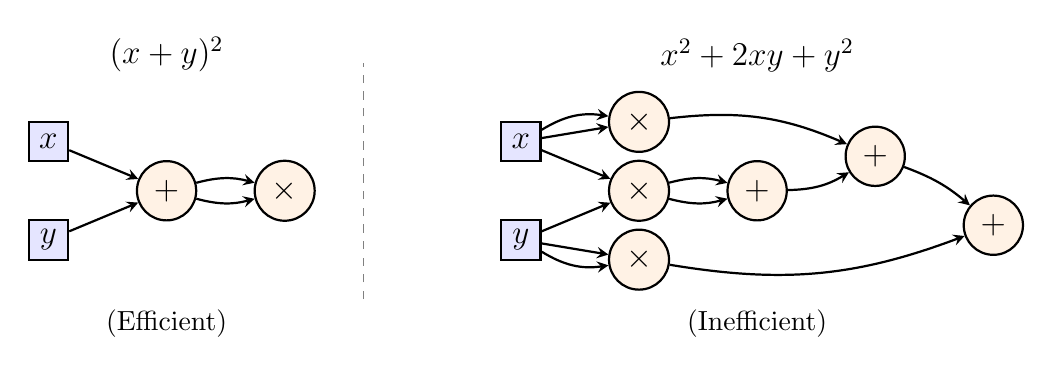
\begin{tikzpicture}[
    scale=0.5,
    op/.style={circle, draw, fill=orange!10, minimum size=0.4cm, thick, font=\large},
    var/.style={rectangle, draw, fill=blue!10, minimum size=0.5cm, thick, font=\large},
    edge/.style={->, >=stealth, thick}
]

% ================= LEFT DIAGRAM =================
\begin{scope}[rotate=-90, transform shape=false]
    \node[var] (x1) at (-5,0) {$x$};
    \node[var] (x2) at (-2.5,0) {$y$};
    \node[op] (add) at (-3.75,3) {$+$};
    \node[op] (mult) at (-3.75,6) {$\times$};
    
    \draw[edge] (x1) -- (add);
    \draw[edge] (x2) -- (add);
    \draw[edge] (add) to[bend left=15] (mult);
    \draw[edge] (add) to[bend right=15] (mult);

    \node[below=1 cm of add] {(Efficient)};
    \node[above=1 cm of add, font=\large] {$(x+y)^2$};
\end{scope}

% ================= SEPARATOR =================
\draw[dashed, gray] (8, 1) -- (8, 7);

% ================= RIGHT DIAGRAM =================
\begin{scope}[shift={(12,0)}, rotate=-90, transform shape=false]
    \node[var] (rx) at (-5,0) {$x$};
    \node[var] (ry) at (-2.5,0) {$y$};

    \node[op] (mx2) at (-5.5,3) {$\times$};
    \node[op] (mxy) at (-3.75,3) {$\times$};
    \node[op] (my2) at (-2,3) {$\times$};

    \node[op] (radd1) at (-3.75,6) {$+$};
    \node[op] (radd2) at (-4.625,9) {$+$};
    \node[op] (radd3) at (-2.875,12) {$+$};

    \draw[edge] (rx) -- (mx2);
    \draw[edge] (rx) to[bend left=20] (mx2);

    \draw[edge] (rx) -- (mxy);
    \draw[edge] (ry) -- (mxy);

    \draw[edge] (ry) -- (my2);
    \draw[edge] (ry) to[bend right=20] (my2);

    \draw[edge] (mxy) to[bend left=15] (radd1);
    \draw[edge] (mxy) to[bend right=15] (radd1);

    \draw[edge] (mx2) to[bend left=15] (radd2);
    \draw[edge] (radd1) to[bend right=15] (radd2);

    \draw[edge] (radd2) to[bend left=10] (radd3);
    \draw[edge] (my2) to[bend right=15] (radd3);

    \node[below=1 cm of radd1] {(Inefficient)};
    \node[above=1 cm of radd1, font=\large] {$x^2 + 2xy + y^2$};
\end{scope}

\end{tikzpicture}
\end{center}

Many polynomials admit small arithmetic circuits because they can be computed by reusing intermediate subexpressions. A first example is the \textit{Horner scheme} \citep{Horner1819NewMethod}. Given a univariate polynomial
\(
p(x)=\sum_{i=0}^{d} a_i x^i,
\)
one may evaluate $p$ by the decreasing recurrence
\(
t_d=a_d,\qquad t_i=a_i + x\cdot t_{i+1}\quad (i=d-1,\dots,0),
\)
so that $p(x)=t_0$. This recursion is equivalent to the nested expression
\[
p(x)=a_0 + x\bigl(a_1 + x( a_2 + \cdots + x(a_{d-1}+x a_d)\cdots )\bigr).
\]
Horner's method uses exactly $d$ addition and $d$ multiplication gates, in contrast to the naive circuit $\sum_i a_i x^i$ which recomputes powers $x^i$ for each term. 

A multivariate example is provided by \textit{elementary symmetric polynomials}. The elementary symmetric polynomial of degree $k$ in $n$ variables is
\[
e_k(x_1,\dots,x_n)=\sum_{1\le i_1<\cdots<i_k\le n} x_{i_1}\cdots x_{i_k},
\]
and it satisfies the recurrence
\[
e_k(x_1,\dots,x_n)=e_k(x_1,\dots,x_{n-1}) + x_n\cdot e_{k-1}(x_1,\dots,x_{n-1}).
\]
This recurrence expresses $e_k$ in terms of two previously computed polynomials on $(n-1)$ variables.

The arithmetic circuit problem is central in algebraic complexity theory. Valiant \citep{Valiant1979CompletenessClasses} defined the class $\mathrm{VP}$, which consists of families of polynomials computable by arithmetic circuits of polynomial size in terms the parameter. Valiant's $\mathrm{VNP}$ class is an algebraic analogue of $\mathrm{NP}$. Valiant then showed that computing the \textit{permanent polynomials}

\[\operatorname{per}_n\left(x_{i,j}\right)=\sum_{\sigma \in S_n} \prod_{i=1}^n x_{i, \sigma(i)}, \quad  (i,j) \in [n] \times [n]\]
is $\mathrm{VNP}$-complete \citep{Valiant1979Permanent}.





\subsection{AlphaZero-Style Search and Policy Optimization}

AlphaZero's achievement was its ability to master two-player perfect information games (such as Go, chess, shogi) \citep{Silveretal2018AlphaZero}. AlphaZero combined a neural network with the MCTS framework, allowing the agent to master gameplay through self-play only without any human feedback/input beyond the rules of the game. Central to the approach is a single neural network that outputs both a policy (probability distribution over moves to choose) and a value estimate (predicted outcome from a given state), which together guide the tree search.

\paragraph{\underline{Monte Carlo Tree Search}}

The Monte-Carlo Tree Search algorithm is a powerful search algorithm that samples value-based trajectories to incrementally build a search tree. It balances exploration and exploitation using upper confidence bounds (UCB)  \citep{KocsisBanditMonteCarlo}. For a state-action pair $(s,a)$, one has $$\text{UCB}(s, a) = \frac{Q(s, a)}{N(s, a)} + c \sqrt{\frac{\ln N(s)}{N(s, a)}},$$

where $Q(s, a)$ is the total value, $N(s, a)$ is the visit count for that action, $N(s)$ is the parent visit count, and $c$ is an exploration constant that balances exploitation of high-value actions with exploration of less-visited nodes.

The algorithm proceeds in four phases: selection, where the tree is traversed using UCB; expansion, where a new node is added; rollout, where the value of the new node is estimated; and backpropagation, where statistics are updated along the visited path.

The sequential nature of circuit construction (selecting one gate at a time) maps naturally onto MCTS's tree structure, making it well-suited for navigating the combinatorial search space of arithmetic circuits.

\paragraph{\underline{Proximal Policy Optimization}}

Proximal Policy Optimization (PPO) is a policy-gradient reinforcement learning method, its key idea is that it stabilizes training by preventing the policy to change drastically in a single update step. The core equation of PPO is a clipped surrogate function \citep{schulman2017ppo} $$L^{\text{CLIP}}(\theta) = \mathbb{E}\left[ \min\left(r_t(\theta)\hat{A}_t, \text{clip}(r_t (\theta), 1 - \epsilon, 1 + \epsilon)\hat{A}_t)\right) \right],$$

where $r_t(\theta) = \frac{\pi_\theta(a_t|s_t)}{\pi_{\theta_{\text{old}}}(a_t|s_t)}$ is the probability ratio between the new and old policies, $\hat{A}_t$ is the estimated advantage and $\epsilon$ is a clipping hyperparmeter which helps prevent updates that are unhelpfully large.

In our work, we implemented PPO as the training algorithm for the neural network. This replaces AlphaZero's original implementation of the policy iteration scheme. PPO's training stability is particularly valuable in our setting, where the reward landscape of circuit construction is sparse and sensitive to large policy shifts.

Together, the neural network trained via PPO provides the policy prior and value estimates that guide MCTS, while the improved action distributions produced by MCTS serve as training targets for the network to choose the best action.

\paragraph{\underline{Soft Actor-Critic}}

SAC is an off-policy actor-critic method that adds the standard RL objective function with an entropy bonus which encourages the agent to continue exploration. SAC employs twin Q-networks to reduce overestimation bias, along with a learnable temperature parameter $\alpha$ that balances how much the agent prioritizes rewards vs. exploration \citep{Haarnoja2018SAC}. The SAC objective function is $$J(\pi) = \sum_t \mathbb{E}\left[ r(s_t, a_t) + \alpha H(\pi(\cdot | s_t)) \right],$$ where $H$ is the entropy of the policy. The agent's goal is to maximize the reward while also keeping its policy stochastic. In our work, the circuit construction has sparse rewards, so the agent might not know if it's on the right track until many steps are taken, and SAC's entropy regularization helps maintain exploration in this setting. While SAC was originally designed for continuous action spaces, we adapt it to discrete settings \citep{christodoulou2019sacdiscrete}.

% \paragraph{\underline{Transformer}}

% Transformers are sequence-to-sequence models that process large sequences of data in parallel instead of sequentially using a mechanism called ``attention" \citep{vaswani2017attention}. These models have also been shown to successfully learn mappings between symbolic mathematical expressions \citep{Lample2020Deep}. The success in learning symbolic mappings suggests that the problem of circuit discovery, finding a sequence of operations that computes a target polynomial, may also be amenable to a supervised sequence-to-sequence approach.



\section{Methodology}
\label{sec:methods}
\subsection{Environment and State Encoding}

We model arithmetic circuit construction as a single-player Markov Decision Process (MDP), where the state is a partially-built circuit represented as a directed acyclic graph (DAG), actions correspond to selecting an operation and two existing nodes, and transitions deterministically append a new node to the graph. The agent's goal is to reach a state where one of the computed nodes matches the target polynomial, in as few steps as possible.

Formally, let $\mathcal{G}_t = (V_t, E_t)$ denote the circuit graph at step $t$, with initial nodes $V_0 = \{x_0, \ldots, x_{n-1}, 1\}$ consisting of the input variables and a constant. At each step the agent selects an action $a_t = (\star, v_i, v_j)$ where $\star \in \{+, \times\}$ and $v_i, v_j \in V_t$, producing a new node $v_{\text{new}}$ that computes $v_i \star v_j$. The transition updates the graph as $V_{t+1} = V_t \cup \{v_{\text{new}}\}$.

Each node $v \in V_t$ is represented by a 4-dimensional feature vector consisting of a 3-bit one-hot encoding for node type (input variable, constant, or operation result) and a scalar value, with directed edges connecting operand nodes to their result nodes and self-loops added for message passing. The target polynomial is not represented symbolically but as a compact circuit encoding. This encoding concatenates operation-type one-hots, edge-selection one-hots, and a last-generated-node indicator derived from a reference action sequence. The action space is also flattened, so each action $a_t = (\star, v_i, v_j)$ is mapped to a unique integer index. Invalid actions (referencing nodes that are not yet created) are masked out at each step.

\subsection{Game-Board Generation}

To generate structured training data, we construct a game-board: a directed acyclic graph that enumerates all polynomials reachable from the input variables within $\mathcal{C}$ arithmetic operations. We start with seed nodes $V_0 = \{x_0, \ldots, x_{n-1}, 1\}$,  and at each step every pair of existing nodes is combined via addition and multiplication, and each distinct resulting polynomial becomes a new node. In this DAG, edges represent arithmetic operations, and the step at which a node first appears corresponds to the minimum number of gates needed to compute that polynomial. To control the combinatorial growth of the DAG, we cap the number of expansion steps at $\mathcal{C}$. 

Not all polynomials in the DAG are equally useful for training. Some have only one path from the seed nodes (one unique optimal circuit), meaning the agent has no real choice to learn. We say that a polynomial is \textit{interesting} if it admits multiple distinct shortest paths in the DAG, meaning multiple optimal circuits exist. These targets force the agent to learn meaningful decision-making rather than memorizing a single forced sequence.

To better understand the structure of the resulting search space, we analyze basic statistics of the generated C4 game-board DAG. In this graph, a circuit corresponds to a path from a root node in $V_0$ to a target polynomial, and an \textit{optimal circuit} is defined as a shortest such path. Because multiple arithmetic sequences can produce the same polynomial, many nodes admit several distinct optimal circuits.

Table \ref{tab:c4_depth} reports the distribution of nodes by circuit depth (the minimum number of arithmetic operations required to produce the polynomial). Most nodes appear at depths three and four, reflecting the rapid combinatorial growth of reachable polynomials as operations are composed. Importantly, the step index used during board construction exactly matches the shortest-path depth in the DAG, meaning that nodes are discovered precisely when their minimal circuit first becomes available.

Table \ref{tab:c4_summary} summarizes structural properties of the generated graphs. In both the two-variable (C4-main) and single-variable (C4-pretrain) boards, the vast majority of nodes admit multiple optimal circuits. This confirms that the environment contains substantial decision freedom rather than forcing a single computation sequence. Some nodes admit dozens or even hundreds of optimal circuits, while the total number of possible circuits can be much larger when non-optimal paths are included.


\begin{table}[t]
\centering
\small
\begin{tabular}{lcc}
\toprule
Depth distribution (nodes by step) & C4-main & C4-pretrain \\
\midrule
0 & 3 & 1 \\
1 & 12 & 2 \\
2 & 174 & 9 \\
3 & 10{,}862 & 96 \\
4 & 8{,}949 & 6{,}548 \\
\bottomrule
\end{tabular}
\caption{Circuit-depth distribution for C4 boards.}
\label{tab:c4_depth}
\end{table}


\begin{table}[t]
\centering
\small
\begin{tabular}{lcc}
\toprule
Metric & C4-main (multivar) & C4-pretrain (single-var) \\
\midrule
Nodes & 20{,}000 & 6{,}656 \\
Edges & 31{,}746 & 20{,}966 \\
Roots & 3 & 1 \\
Nodes with multiple optimal circuits & 18{,}966 (94.83\%) & 6{,}592 (99.04\%) \\
Max optimal circuits for one node & 164 & 92 \\
Max total circuits for one node & 1{,}596 & 15{,}296 \\
\bottomrule
\end{tabular}
\caption{C4 game-board structure and path-efficiency statistics. Optimal circuits are shortest root-to-node paths.}
\label{tab:c4_summary}
\end{table}

\subsection{PPO + MCTS}

Our primary agent, CircuitBuilder, combines graph-based state encoding with a Transformer decoder to produce both a policy and value estimate. The GNN encoder processes the circuit DAG. It uses GCNConv layers with residual connections and layer normalization, and the per-node embeddings are aggregated via a global mean pooling into a single graph embedding vector. The target polynomial is encoded using a compact one-hot scheme that concatenates operation-type indicators, edge-selection indicators, and a last-generated-node indicator from a reference action sequence. This is then projected through a linear layer into the same embedding dimension. A Transformer decoder then attends over both embeddings: a learnable output token serves as the query, while the graph embedding and target polynomial embedding are stacked to form the decoder memory. The decoder output is passed to a policy head, which produces logits over the action space masked to valid actions, and a value head, which outputs a scalar estimate of the current state's value.

\paragraph{\underline{Supervised Pretraining}}

We first train on (state, next-action) pairs extracted from known optimal circuits from the game board, where each intermediate step of a circuit becomes a training example. The model is trained to minimize cross-entropy loss on action predictions plus mean squared error on value predictions. This creates a strong policy initialization before RL fine-tuning.

\paragraph{\underline{PPO Fine-Tuning}}

After supervised pretraining, we fine-tune the model using PPO. Using Generalized Advantage Estimation (GAE) to compute low-variance advantage estimates. $$\delta_t = r_t + \gamma V(s_{t+1}) - V(s_t), \qquad \hat{A}_t = \delta_t + \gamma \lambda \hat{A}_{t+1}.$$
Here, $\gamma$ is the discount factor and $\lambda$ controls the bias-variance tradeoff. The full PPO loss function that we optimize is $$\mathcal{L}_{\text{PPO}}(\theta) = -\mathbb{E}\left[\min\left(r_t(\theta)\hat{A}_t, \text{clip}(r_t(\theta), 1-\epsilon, 1+\epsilon)\hat{A}_t\right)\right] + c_v \text{MSE}(V_\theta(s_t), \hat{R}_t) - c_e \mathbb{E}[\mathcal{H}(\pi_\theta(\cdot|s_t))].$$

The three terms are the clipped surrogate objective, a value function loss, and an entropy bonus that encourages exploration. We employ a curriculum learning strategy: training begins at polynomial complexity 1, and the complexity increases when the agent's success rate exceeds a threshold over a sliding window.

\paragraph{\underline{MCTS Integration}}

During PPO data collection, MCTS optionally guides action selection. We employ the Bernoulli mixing scheme: $$a_t = \begin{cases} a_t^{\text{MCTS}}, & z_t = 1 \\ a_t^{\pi}, & z_t = 0 \end{cases}, \quad z_t \sim \text{Bernoulli}(p_{\text{mix}}).$$

With probability $p_\text{mix}$ the agent defers to the MCTS planner, otherwise it samples from its own policy. Our MCTS uses the neural network's value head to evaluate leaf nodes (AlphaZero-style), replacing random rollouts with learned value estimates. It returns the action with the highest visit count. This exposes the policy network to higher-quality trajectories during training, improving sample efficiency over pure policy sampling.
\subsubsection{MCTS-Guided Expert Iteration}
During the data collection phase, we employ an Expert Iteration framework that hybridizes Monte Carlo Tree Search (MCTS) with PPO. Rather than relying solely on the policy network for exploration, the agent utilizes MCTS as an "expert" planner to generate higher-quality trajectory data. 

At each timestep $t$, the MCTS search is guided by the current policy-value network, producing a visit-count distribution $\pi_{MCTS}$. To balance early-episode exploration with later-episode exploitation, action selection is tempered by a decaying temperature parameter $\tau$:
$$
\tau(t) = \tau_{final} + (\tau_{init} - \tau_{final}) \max \left(1 - \frac{t}{t_{decay}}, 0 \right)
$$
where $t_{decay}$ defines the annealing schedule.

A critical architectural distinction in our approach lies in the formulation of the PPO importance sampling ratio. Standard AlphaZero implementations train the policy head to minimize the cross-entropy loss against the MCTS visit counts. In our PPO formulation, the surrogate objective relies on the probability ratio:
$$
r_t(\theta) = \frac{\pi_{\theta}(a_t|s_t)}{\pi_{\theta_{old}}(a_t|s_t)}
$$
Crucially, the denominator $\pi_{\theta_{old}}(a_t|s_t)$ is the probability assigned by the \textit{network's own policy} at the time of data collection, not the probability derived from the MCTS visit counts. If the MCTS probabilities were used in the denominator, the ratio $r_t(\theta)$ would remain near $1$ (as the MCTS search is already anchored by the prior $\pi_\theta$), resulting in a near-zero policy gradient. 

By using the network's internal logits for the baseline ratio, MCTS acts strictly as a data-quality enhancer—finding shorter, more efficient circuit paths—while the clipped PPO objective provides stable, meaningful updates to the network parameters to approximate this improved behavior. Furthermore, the Generalized Advantage Estimation (GAE) targets are bootstrapped using the network's value head $V_\theta(s)$, rather than the MCTS value estimates, ensuring consistent variance reduction during the PPO update.

% \subsubsection{Ablation Studies}
% To understand the contribution of the MCTS hybrid approach, we define several ablation conditions:
% \begin{itemize}
%     \item \textbf{Pure PPO (No MCTS):} The agent samples actions directly from the policy network $\pi_\theta$ without look-ahead search, isolating the impact of MCTS on sample efficiency.
%     \item \textbf{MCTS-Denominator PPO:} The PPO importance ratio is calculated using $\pi_{MCTS}(a_t|s_t)$ as the old policy denominator. We hypothesize this will result in collapsed policy gradients and poor learning.
%     \item \textbf{Pure AlphaZero:} Replacing the PPO clipped surrogate objective entirely with the standard cross-entropy loss against MCTS visit counts, to evaluate the necessity of PPO's conservative policy steps in the sparse-reward circuit environment.
% \end{itemize}


\subsection{Soft Actor-Critic}

SAC method shares the same GNN-Transformer backbone as CircuitBuilder, but it replaces the single value head with twin Q-heads that output per-action Q-values. The SAC is off-policy, storing transitions in a replay buffer and using soft target network updates via Polyak averaging. The full update procedure is given in Algorithm~\ref{alg:sac} \citep{OpenAISAC}.

\begin{algorithm}[h]
\caption{Discrete SAC with MCTS Distillation}
\label{alg:sac}
\begin{algorithmic}[1]
\REQUIRE Replay buffer $\mathcal{B}$, policy network $\pi_\theta$, twin Q-networks $Q_{\theta,1}, Q_{\theta,2}$, target networks $Q_{\bar{\theta},1}, Q_{\bar{\theta},2}$, temperature $\alpha$, MCTS coefficient $\lambda_{\text{mcts}}$, soft update rate $\tau$
\FOR{each update step}
    \STATE Sample minibatch $\{(s_t, a_t, r_t, s_{t+1}, d_t, \pi^{\text{MCTS}}_t, m_t)\} \sim \mathcal{B}$
    \STATE \textit{// Compute soft value target over valid actions}
    \STATE $V_{\bar{\theta}}(s') \leftarrow \sum_{a \in \mathcal{A}_{\text{valid}}(s')} \pi_\theta(a|s')\left(\min_i Q_{\bar{\theta},i}(s',a) - \alpha \log \pi_\theta(a|s')\right)$
    \STATE $y_t \leftarrow r_t + \gamma(1 - d_t)\, V_{\bar{\theta}}(s_{t+1})$
    \STATE \textit{// Update twin Q-networks}
    \STATE $\mathcal{L}_Q \leftarrow \text{MSE}(Q_{\theta,1}(s_t, a_t),\, y_t) + \text{MSE}(Q_{\theta,2}(s_t, a_t),\, y_t)$
    \STATE \textit{// Update policy over valid actions}
    \STATE $\mathcal{L}_\pi \leftarrow \mathbb{E}_{s_t}\!\left[\sum_{a \in \mathcal{A}_{\text{valid}}} \pi_\theta(a|s_t)\left(\alpha \log \pi_\theta(a|s_t) - \min_i Q_{\theta,i}(s_t, a)\right)\right]$
    \IF{MCTS distribution available ($m_t = 1$)}
        \STATE $\mathcal{L}_{\text{CE}} \leftarrow -\mathbb{E}_{s_t}\!\left[\sum_a \pi^{\text{MCTS}}(a|s_t) \log \pi_\theta(a|s_t)\right]$
    \ELSE
        \STATE $\mathcal{L}_{\text{CE}} \leftarrow 0$
    \ENDIF
    \STATE $\mathcal{L}_{\text{total}} \leftarrow \mathcal{L}_Q + \mathcal{L}_\pi + \lambda_{\text{mcts}}\, \mathcal{L}_{\text{CE}}$
    \STATE Update $\theta$ by minimizing $\mathcal{L}_{\text{total}}$
    \STATE $\bar{\theta} \leftarrow (1 - \tau)\bar{\theta} + \tau\theta$
\ENDFOR
\end{algorithmic}
\end{algorithm}

We employ the same curriculum learning strategy as PPO, with the addition that complexity can also decrease when the success rate falls below a lower threshold, preventing the agent from stalling on targets beyond its current capability.

% \subsection{Polynomial-to-Circuit Transformer}

% This approach treats circuit discovery as a translation task, using a standard encoder-decoder Transformer rather than the GNN and Transformer architecture used by the RL agents. The model is a standard Transformer with learned character embeddings and sinusoidal positional encodings. The model operates at the character level, with the input being the expanded polynomial string and the output being a circuit expression that preserves the structure of the shortest-path construction. The training data consists of polynomial-circuit pairs derived from the game-board's shortest-path action sequences, which are converted to SymPy expression strings. The training objective is implemented as token-level cross-entropy with teacher forcing: $$\mathcal{L}_{\text{TF}}(\theta) = -\sum_{t=1}^{m-1} \log p_\theta(y_{t+1} \mid y_{1:t}, x_{1:n}).$$

% At inference time, circuits are produced via greedy autoregressive decoding, with correctness verified via SymPy algebraic equivalence rather than string matching. Unlike the RL methods which learn through exploration, this is a purely supervised approach that requires access to optimal circuit constructions during training. 








\section{Results}
\label{sec:results}

We trained PPO+MCTS and SAC on an AWS EC2 cloud machine with an NVIDIA Tesla T4 GPU (16\,GB). Both models use a GNN encoder with \texttt{GCNConv} layers to process the circuit DAG, fused with a target polynomial embedding, and output policy logits and value estimates. We evaluate performance on fixed-complexity targets at $C=5$ and $C=6$ (two variables over $\mathbb{F}_5$). Training curves are provided in \Cref{apx:plots}.

For a target polynomial $f$, we declare \emph{success} if the agent produces an arithmetic circuit whose output polynomial equals $f$. Tables~\ref{tab:ppo_summary} report training metrics for PPO+MCTS over 200 iterations with batch size 256.

\begin{table}[h]
\centering
\caption{PPO+MCTS training summary at $C=5$ and $C=6$ (two variables over $\mathbb{F}_5$, batch size 256). Success rates are percentages; entropy is over the action space.}
\label{tab:ppo_summary}
\begin{tabular}{l c c c c c}
\toprule
Task & Iter 50 & Iter 100 & Iter 150 & Iter 200 & Entropy \\
\midrule
$C=5$ success (\%) & 31.25 & 26.95 & 35.55 & \textbf{35.94} & 3.28 \\
$C=6$ success (\%) & 19.53 & 20.31 & 24.61 & 25.39 & 3.28 \\
\midrule
$C=5$ avg reward   & 2.693 & 2.245 & 3.131 & 3.181 & --- \\
$C=6$ avg reward   & 1.485 & 1.541 & 2.021 & 2.137 & --- \\
\bottomrule
\end{tabular}
\end{table}

PPO+MCTS reaches approximately $36\%$ success rate on $C=5$ targets and approximately $25\%$ on $C=6$ targets after 200 iterations. The entropy remains stable near $3.3$ throughout training, indicating sustained exploration without policy collapse. The value function loss decreases over training, suggesting the network learns meaningful state valuations.

The performance gap between $C=5$ and $C=6$ reflects the combinatorial growth of the search space. Although $C=6$ targets require only one additional operation, the number of reachable polynomials grows super-exponentially with circuit depth.

\paragraph{\underline{Discussion \& Future Directions}}
PPO combined with MCTS achieves the highest success rates across both complexity levels. SAC converges quickly but plateaus at a lower success rate, suggesting it struggles to convert exploration into consistent task completion. This gap indicates that SAC may need better reward shaping or curriculum design to fully leverage its strengths in sparse-reward settings. Future work includes scaling to higher complexity targets ($C \geq 7$), improving reward shaping through factor-aware subgoal decomposition, and training across multiple complexity levels simultaneously via curriculum learning. Improved representations for polynomials and circuits remain an important direction.

Our experiments focus on small circuits (two variables and at most six gates). While this scale is far smaller than the polynomial families studied in algebraic complexity theory, it provides a controlled setting for evaluating whether reinforcement learning can discover efficient circuit constructions. The goal of this work is to study learning behavior on small instances before attempting to scale to larger circuits and higher-variable polynomials in future work.

\subsubsection*{Acknowledgments}
This project is a part of the UW Math AI Lab. We thank the UW eScience School for computing resources. CPU and GPU computing were in part done using AWS credits from the UW eScience School and UW IT, and also in part done using the UW Research Computing Club funded from the UW Student Technology Fee Committee. Some parts of the code base are produced with the help of GitHub Copilot.

\appendix

\section{Training Plots}
\label{apx:plots}
\begin{figure}[h]
    \centering
    \includegraphics[width=.7\linewidth]{PPO+MCTS.png}
    \caption{Loss curves and success rates for PPO + MCTS in training.}
    \label{fig:PPO}
\end{figure}

\begin{figure}[h]
    \centering
    
\includegraphics[width=.9\linewidth]{sac_v4_live_smooth.png}
    \caption{Soft Actor-Critic Training Metrics Over Time (MA50) at Complexity level 1-4}
    \label{fig:SAC}
\end{figure}

% \section{Training Plots}
% \label{apx:plots}
% \begin{figure}[h]
%     \centering
%     \includegraphics[width=.7\linewidth]{PPO+MCTS.png}
%     \caption{Loss curves and success rates for PPO + MCTS in training.}
%     \label{fig:PPO}
% \end{figure}


% \begin{figure}[h]
%     \centering
%     
\includegraphics[width=.9\linewidth]{sac_v4_live_smooth.png}
%     \caption{Soft Actor-Critic Training Metrics Over Time (MA50) at Complexity level 1-4}
%     \label{fig:SAC}
% \end{figure}

% \begin{figure}[h]
%     \centering
%     
\includegraphics[width=0.4\linewidth]{ICLR 2026 - Workshop/board_C4.training.png}
%     \caption{Training and Validation plot of Transformer at Complexity level 4}

% \label{fig:transformerC4}
% \end{figure}

\end{document}